\documentclass[10pt]{beamer}

\usepackage[english]{babel}
\usepackage[utf8]{inputenc}
\usepackage{lmodern}
\usepackage{listings}
\usepackage{caption}
\usepackage{subcaption}

\captionsetup[lstlisting]{ margin=0pt }

\definecolor{lgray}{gray}{0.96}
\definecolor{lbcolor}{rgb}{0.9,0.9,0.9}
\lstset{
    framesep=2pt,
    basicstyle=\ttfamily,
    breaklines=true,
    breakatwhitespace=true,
    aboveskip={0.75\baselineskip},
    columns=fixed,
    showstringspaces=false,
    breaklines=true,
    frame=single,
    rulecolor=\color{lgray},
    showtabs=false,
    showspaces=false,
    showstringspaces=false,
    backgroundcolor=\color{lgray},
    identifierstyle=\ttfamily,
    keywordstyle=\color[rgb]{0,0,1},
    commentstyle=\color[rgb]{0.0,0.26,0.15},
    stringstyle=\color[rgb]{0.627,0.126,0.941}
}

\setbeamertemplate{caption}[numbered]
\setbeamersize{text margin left=5mm,text margin right=5mm}


\usetheme{AGH}

\begin{document}


\begin{frame}
\frametitle{Improved documentation}
\begin{itemize}
    \item Short documentation (usage description) for \emph{gitio} has been created.
    \item \emph{Gitio} is our tool for managing Git submodules.
\end{itemize}
\begin{figure}
    \centering 
    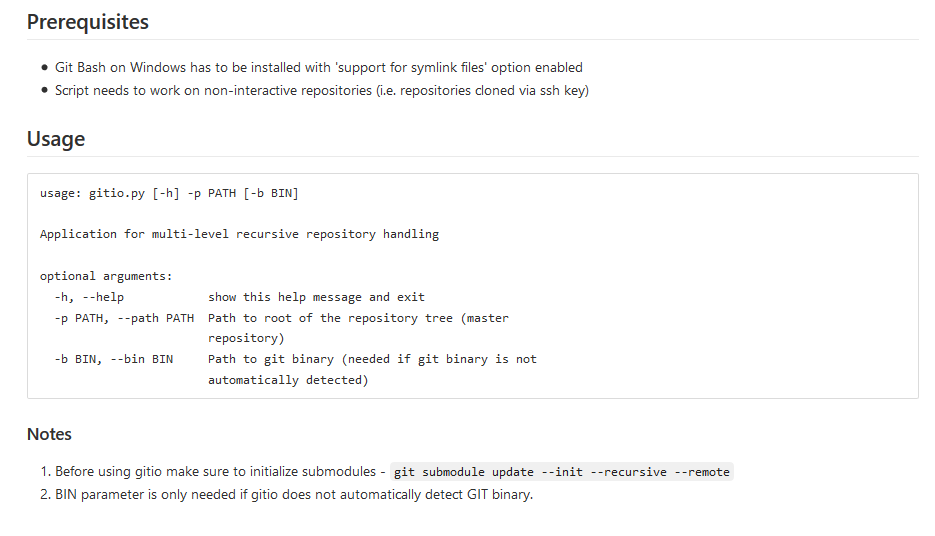
\includegraphics[width=0.75\textwidth]{static/gitio_documentation.PNG}
\end{figure}
\end{frame}

\begin{frame}
\frametitle{Custom artifacts for releases}
\begin{itemize}
    \item Automated versioning has been improved and finished. 
    \item Compiled applications (and driver) are now part of generated releases.
    \item They can now be downloaded directly from GitLab.
\end{itemize}
\begin{figure}
    \centering 
    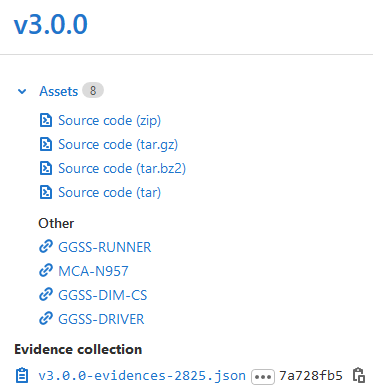
\includegraphics[width=0.4\textwidth]{static/artifacts.png}
\end{figure}
\end{frame}

\begin{frame}
\frametitle{HV management commands refactoring}
\begin{itemize}
    \item More user-friendly commands for HV management using DIM.
    \item GET (MON) and SET command changed (no need to send raw HV commands).
    \item Example syntax: \lstinline{hv 0:* mon vmon}.
    \item \lstinline{*} - all channels (or modules).
    \item Still work in progress.
\end{itemize}
\end{frame}


\begin{frame}
\frametitle{Current plans}
\begin{itemize}
    \item Single RPM with all GGSS applications and utilities (for fast and easy deploy).
    \item Hardware testing scripts refactoring and upgrade (yaml based scenarios).
    \item Additional documentatiom improvements (GitLab CI tasks debugging).
    \item Further code refactoring.
    \item GGSS improvements, for example peak finding / range fitting.
\end{itemize}
\end{frame}
    


\end{document}